\documentclass[finnish,]{book}
\usepackage{lmodern}
\usepackage{amssymb,amsmath}
\usepackage{ifxetex,ifluatex}
\usepackage{fixltx2e} % provides \textsubscript
\ifnum 0\ifxetex 1\fi\ifluatex 1\fi=0 % if pdftex
  \usepackage[T1]{fontenc}
  \usepackage[utf8]{inputenc}
\else % if luatex or xelatex
  \ifxetex
    \usepackage{mathspec}
  \else
    \usepackage{fontspec}
  \fi
  \defaultfontfeatures{Ligatures=TeX,Scale=MatchLowercase}
\fi
% use upquote if available, for straight quotes in verbatim environments
\IfFileExists{upquote.sty}{\usepackage{upquote}}{}
% use microtype if available
\IfFileExists{microtype.sty}{%
\usepackage{microtype}
\UseMicrotypeSet[protrusion]{basicmath} % disable protrusion for tt fonts
}{}
\usepackage[margin=1in]{geometry}
\usepackage{hyperref}
\hypersetup{unicode=true,
            pdftitle={Korrespondenssianalyysi - graafinen ja geometrinen data-analyysin menetelmä},
            pdfauthor={Jussi Hirvonen},
            pdfborder={0 0 0},
            breaklinks=true}
\urlstyle{same}  % don't use monospace font for urls
\ifnum 0\ifxetex 1\fi\ifluatex 1\fi=0 % if pdftex
  \usepackage[shorthands=off,main=finnish]{babel}
\else
  \usepackage{polyglossia}
  \setmainlanguage[]{finnish}
\fi
\usepackage{natbib}
\bibliographystyle{apalike}
\usepackage{color}
\usepackage{fancyvrb}
\newcommand{\VerbBar}{|}
\newcommand{\VERB}{\Verb[commandchars=\\\{\}]}
\DefineVerbatimEnvironment{Highlighting}{Verbatim}{commandchars=\\\{\}}
% Add ',fontsize=\small' for more characters per line
\usepackage{framed}
\definecolor{shadecolor}{RGB}{248,248,248}
\newenvironment{Shaded}{\begin{snugshade}}{\end{snugshade}}
\newcommand{\AlertTok}[1]{\textcolor[rgb]{0.94,0.16,0.16}{#1}}
\newcommand{\AnnotationTok}[1]{\textcolor[rgb]{0.56,0.35,0.01}{\textbf{\textit{#1}}}}
\newcommand{\AttributeTok}[1]{\textcolor[rgb]{0.77,0.63,0.00}{#1}}
\newcommand{\BaseNTok}[1]{\textcolor[rgb]{0.00,0.00,0.81}{#1}}
\newcommand{\BuiltInTok}[1]{#1}
\newcommand{\CharTok}[1]{\textcolor[rgb]{0.31,0.60,0.02}{#1}}
\newcommand{\CommentTok}[1]{\textcolor[rgb]{0.56,0.35,0.01}{\textit{#1}}}
\newcommand{\CommentVarTok}[1]{\textcolor[rgb]{0.56,0.35,0.01}{\textbf{\textit{#1}}}}
\newcommand{\ConstantTok}[1]{\textcolor[rgb]{0.00,0.00,0.00}{#1}}
\newcommand{\ControlFlowTok}[1]{\textcolor[rgb]{0.13,0.29,0.53}{\textbf{#1}}}
\newcommand{\DataTypeTok}[1]{\textcolor[rgb]{0.13,0.29,0.53}{#1}}
\newcommand{\DecValTok}[1]{\textcolor[rgb]{0.00,0.00,0.81}{#1}}
\newcommand{\DocumentationTok}[1]{\textcolor[rgb]{0.56,0.35,0.01}{\textbf{\textit{#1}}}}
\newcommand{\ErrorTok}[1]{\textcolor[rgb]{0.64,0.00,0.00}{\textbf{#1}}}
\newcommand{\ExtensionTok}[1]{#1}
\newcommand{\FloatTok}[1]{\textcolor[rgb]{0.00,0.00,0.81}{#1}}
\newcommand{\FunctionTok}[1]{\textcolor[rgb]{0.00,0.00,0.00}{#1}}
\newcommand{\ImportTok}[1]{#1}
\newcommand{\InformationTok}[1]{\textcolor[rgb]{0.56,0.35,0.01}{\textbf{\textit{#1}}}}
\newcommand{\KeywordTok}[1]{\textcolor[rgb]{0.13,0.29,0.53}{\textbf{#1}}}
\newcommand{\NormalTok}[1]{#1}
\newcommand{\OperatorTok}[1]{\textcolor[rgb]{0.81,0.36,0.00}{\textbf{#1}}}
\newcommand{\OtherTok}[1]{\textcolor[rgb]{0.56,0.35,0.01}{#1}}
\newcommand{\PreprocessorTok}[1]{\textcolor[rgb]{0.56,0.35,0.01}{\textit{#1}}}
\newcommand{\RegionMarkerTok}[1]{#1}
\newcommand{\SpecialCharTok}[1]{\textcolor[rgb]{0.00,0.00,0.00}{#1}}
\newcommand{\SpecialStringTok}[1]{\textcolor[rgb]{0.31,0.60,0.02}{#1}}
\newcommand{\StringTok}[1]{\textcolor[rgb]{0.31,0.60,0.02}{#1}}
\newcommand{\VariableTok}[1]{\textcolor[rgb]{0.00,0.00,0.00}{#1}}
\newcommand{\VerbatimStringTok}[1]{\textcolor[rgb]{0.31,0.60,0.02}{#1}}
\newcommand{\WarningTok}[1]{\textcolor[rgb]{0.56,0.35,0.01}{\textbf{\textit{#1}}}}
\usepackage{longtable,booktabs}
\usepackage{graphicx,grffile}
\makeatletter
\def\maxwidth{\ifdim\Gin@nat@width>\linewidth\linewidth\else\Gin@nat@width\fi}
\def\maxheight{\ifdim\Gin@nat@height>\textheight\textheight\else\Gin@nat@height\fi}
\makeatother
% Scale images if necessary, so that they will not overflow the page
% margins by default, and it is still possible to overwrite the defaults
% using explicit options in \includegraphics[width, height, ...]{}
\setkeys{Gin}{width=\maxwidth,height=\maxheight,keepaspectratio}
\IfFileExists{parskip.sty}{%
\usepackage{parskip}
}{% else
\setlength{\parindent}{0pt}
\setlength{\parskip}{6pt plus 2pt minus 1pt}
}
\setlength{\emergencystretch}{3em}  % prevent overfull lines
\providecommand{\tightlist}{%
  \setlength{\itemsep}{0pt}\setlength{\parskip}{0pt}}
\setcounter{secnumdepth}{5}
% Redefines (sub)paragraphs to behave more like sections
\ifx\paragraph\undefined\else
\let\oldparagraph\paragraph
\renewcommand{\paragraph}[1]{\oldparagraph{#1}\mbox{}}
\fi
\ifx\subparagraph\undefined\else
\let\oldsubparagraph\subparagraph
\renewcommand{\subparagraph}[1]{\oldsubparagraph{#1}\mbox{}}
\fi

%%% Use protect on footnotes to avoid problems with footnotes in titles
\let\rmarkdownfootnote\footnote%
\def\footnote{\protect\rmarkdownfootnote}

%%% Change title format to be more compact
\usepackage{titling}

% Create subtitle command for use in maketitle
\newcommand{\subtitle}[1]{
  \posttitle{
    \begin{center}\large#1\end{center}
    }
}

\setlength{\droptitle}{-2em}

  \title{Korrespondenssianalyysi - graafinen ja geometrinen data-analyysin
menetelmä}
    \pretitle{\vspace{\droptitle}\centering\huge}
  \posttitle{\par}
    \author{Jussi Hirvonen}
    \preauthor{\centering\large\emph}
  \postauthor{\par}
      \predate{\centering\large\emph}
  \postdate{\par}
    \date{Versio 0.07, tulostettu 2018-10-25}


\usepackage{amsthm}
\newtheorem{theorem}{Theorem}[chapter]
\newtheorem{lemma}{Lemma}[chapter]
\theoremstyle{definition}
\newtheorem{definition}{Definition}[chapter]
\newtheorem{corollary}{Corollary}[chapter]
\newtheorem{proposition}{Proposition}[chapter]
\theoremstyle{definition}
\newtheorem{example}{Example}[chapter]
\theoremstyle{definition}
\newtheorem{exercise}{Exercise}[chapter]
\theoremstyle{remark}
\newtheorem*{remark}{Remark}
\newtheorem*{solution}{Solution}
\begin{document}
\maketitle

{
\setcounter{tocdepth}{2}
\tableofcontents
}
\hypertarget{alkutoimia}{%
\chapter*{Alkutoimia}\label{alkutoimia}}
\addcontentsline{toc}{chapter}{Alkutoimia}

Ladataan r-paketit, ei tulosteta dokumenttiin. Pelkkä YAML- `front
matter', lisäkonfiguroinnit tiedostoissa \_bookdown.yml ja \_output.yml.

Dokumettiin kuuluvat Rmd-tiedostot luetellaan eksplisiittisesti
\_bookdown.yml-tiedostossa.

RefWorksistä eksportattu bib-tiedosto kannattaa avata ensin (Atomilla),
ja korjailla skandit jos niissä on vikaa.

\textbf{25.10.18}

\textbf{Ideoita}

\begin{enumerate}
\def\labelenumi{\arabic{enumi}.}
\item
  Ehkä automaattista R-kirjastojen dokumentointia voisi harkita?
\item
  Gitbook-tulosteessa ei saa koodia ``piilotettua'', asetus
  ``code\_folding: hide'' vaatii teeman (theme). \_output.yml -
  tiedostoon lisätty html\_book - formaatti, siinä voi tarvittaessa
  käyttää piilotusta.
\item
  Versiointi: 0.0n aloittelua, 0.n jäsentely koko paperille, 1.n.n
  valmiimpaa tekstiä.
\end{enumerate}

\hypertarget{johdanto}{%
\chapter{Johdanto}\label{johdanto}}

\textbf{xyz} Kirjoitetaan disposition pohjalta, keräillään kaikki
yleiset ca-luonnehdinnat yhteen paikkaan eli johdantoon.

\textbf{Mahdollisia lisäyksiä}

\begin{enumerate}
\def\labelenumi{\arabic{enumi}.}
\item
  Lyhyt esitys CA:n historiasta (vai omaksi luvuksi, luku 2)?
\item
  Käytetyt ohjelmistot, tekninen ympäristö ml. bookdown-asetukset. Ehkä
  paremmin omaksi liitteeksi?
\item
  Tavoitteet, sisältö, rajaukset (jota voi myöhemmin täydentää)
\item
  Muutamat puutteet, onko kerrottava tässä?
\end{enumerate}

\begin{itemize}
\item
  data: ei huomioida sitä, että otoskoot vaihtelevat aika paljon eli
  ``maapainot'' eri suuruisia
\item
  ei huomioida muitakaan otantaan liittyviä asioita (tämä ainakin
  mainittava data-osuudessa)
\item
  kuvaileva menetelmä, mutta mikä on tutkimusongelma? Sellainen pitäisi
  olla.
\end{itemize}

**zxy* Mitä on korrespondenssianalyysi? Muutamalla kappaleella. Yksi
kappale historiasta.

\hypertarget{tutkielman-tavoite-tutkimusongelma}{%
\section{Tutkielman tavoite
(tutkimusongelma?)}\label{tutkielman-tavoite-tutkimusongelma}}

\textbf{zxy} Tässä kerrotaan, miksi tämä työ on kirjoitettu. Esitellään
menetelmä käyttämällä oikeaa dataa. Täsmällisempi esitys sirotellaan
esimerkkiaineiston analyysin tulosten esittelyn lomaan. Pitäisikö tässä
tuoda esille ns. ``ranskalaisen koulukunnan'' matemaattisen perusteiden
korostus, ja data-analyysin filosofia? Ehkä ei, koska sen pohdinta ei
ole pääasia. Se tietysti mainitaan, ja asiaa pohditaan.

\textbf{ks} Esitellään korrespondenssianalyysin käsitteet ja graafisen
analyysin periaatteet.

\textbf{zxy} -mitä ca on? - dimensioiden vähentäminen ja visualisointi -
mihin dataan se soveltuu - määrittele graafinen, deskriptiivinen,
eksploratiivinen data-analyysi - yksinkertainen ca, useamman muuttujan
ca

\textbf{ks} Tämän voi tehdä yksinkertaisen korrespondenssianalyysin
avulla. Yksinkertainen kahden luokittelumuuttujan
korrespondenssianalyysi antaa graafisen analyysin ``\ldots{}perussäännöt
tulkinnalle. Kaikki muut korrespondenssianalyysin muodot ovat saman
algoritmin soveltamista toisen tyyppiisiin datamatriiseihin, ja
tulkintaa sovelletaan vastaavasti (with the consequent adaptation of the
interpretation)''\citep[ , s.
437]{RefWorks:doc:5a857a44e4b0ed2d44664d84}

\textbf{zxy} Miksi eksporatiivinen (määrittele!) ja deskriptiivinen
(määrittele!) menetelmä on esitettävä ``in vivo'', toiminnassa?
Oppikirjoissa (viitteitä) erityisesti MG on havainnolistanut CA:n
matemaattista ja geometristä taustaa synteettisillä aineistoilla. Turha
kopioida tähän. Menetelmän ydin on yksinkertaisen graafisen esityksen --
kartan -- avulla tulkita monimutkaisen empiirisen aineiston muuttujien
riippuvuuksia. Yhteyksiä ei tiivistetä todennäköisyyspäättelyn
kriteereillä tilastolliseen malliin, vaan deskripriivisen analyysin
hengessä esitellään koko aineisto. Mallin sijaan vähennetään
ulottuvuuksia, ja siinä menetetään informaatiota. Tavoitteena on
säilyttää yleensä kaksiulotteisessa kuvassa mahdollisimman suuri osa
alkuperäisen datan vaihtelusta. Eksploratiivinen data-analyysi on
vuoropuhelua aineiston kanssa. Analyysiä tarkennetaan, rajataan ja
muokataan, kun aineisto paljastaa jotain kiinnostavaa tai yllättävää.
Tästä saa jonkinlaisen aasinsillan matriisiyhtälöiden puolustukseksi.
Saksan ja Belgian datan jakaminen on hyvä esimerkki, on ``osattava
tarttua'' menetelmän tulosmatriiseihin.

\textbf{zxy} esitystavan perustelu

\begin{itemize}
\tightlist
\item
  kenelle kirjoitettu? Menetelmästä kiinnostuneelle tilastotieteen ja
  data-analyysin perusteet tuntevalle. R-ohjelmisto ei ole rajoitus,
  SPSS ja SAS sopivat. (SPSS - MG:llä kriittinen huomio ``loose ends -
  paperissa'' tai CAip-teorialiitteessä).
\end{itemize}

\hypertarget{tarkeimmat-lahteet-ja-ohjelmistot}{%
\section{Tärkeimmät lähteet ja
ohjelmistot}\label{tarkeimmat-lahteet-ja-ohjelmistot}}

\textbf{zxy} Tarvitaanko tämä, perustelu? Muutamat lähteet aivan
keskeisiä, ja MG:n kurssi pitää mainita.

\hypertarget{lahteet}{%
\subsection{Lähteet}\label{lahteet}}

Michael Greenacre luennoi lyhyen kurssin korrespondenssianalyysistä
Helsingin yliopistossa keväällä
2017\citep{RefWorks:doc:5b6ef091e4b0984fd9b8c0ca}. Luennot ja
laskuharjoitukset perehdyttivät minut ensimmäistä kertaa tähän
menetelmään, ja kurssin materiaaleihin olen usein palannut. Niihin voi
tutustua Helsingin yliopiston {[}Moodle-palvelussa{]}
(\url{https://moodle.helsinki.fi}) (käyttäjätunnus vaaditaan).
Greenacren kärsivällisesti kirjoitetut perusoppikirjat ovat tehneet
menetelmää laajasti tunnetuksi englantia lukeville.

Ranskalaisen lähestymistan
perusoppikirja\citep{RefWorks:doc:5a857a43e4b0ed2d44664d75} esittelee
menetelmän matemaattiset perusteet. Lyhyt historiallinen katsaus ja
menetelmä soveltamisen perusajatusten esittely valaisevat ranskaa
taitamattomalle data-analyysin koulukunnan ideoita. Kirjoittajat
esittelevät perusteellisesti joitain empiirisiä tutkimuksia, ja lyhyt
mutta naseva matriisilaskennan kritiikki on hyvä panna merkille.

Korrespondenssianalyysi tuli osaksi suomalaista Survo-ohjelmistoa jo
vuonna (\textbf{????}), ja menetelmää on esitelty ainakin kahdessa
oppikirjassa\citep{RefWorks:doc:5a857a44e4b0ed2d44664d95} ja
\citep{RefWorks:doc:5a857a44e4b0ed2d44664da4}.

\hypertarget{kaytetyt-ohjelmistot}{%
\subsection{Käytetyt ohjelmistot}\label{kaytetyt-ohjelmistot}}

\textbf{zxy} R, ca-paketti. löytyy myös muita paketteja.
Rmarkdown\citep{RefWorks:doc:5b6b346fe4b0c619b11b8a3e}, ja bookdown
(\citep{RefWorks:doc:5b6b36dde4b09b7ec442bf8b} ja toinen viite
\citep{R-bookdown}). Mikäs tuo jälkimmäinen on? PDF-lähdeluettelossa ei
ole url-osoitteita.

\textbf{zxy} Helposti toistettavan tutkimukset periaatteet

\begin{enumerate}
\def\labelenumi{\arabic{enumi}.}
\tightlist
\item
  Datasta (löytyy netistä, samoin kattava dokumentaatio) lyhyt matka
  analyysiin.
\item
  Koodi selkeää ja dokumentoitua
\item
  R, LaTeX, pandoc - versiot dokumentoidaan
\end{enumerate}

Tarkemmin liittessä.

\hypertarget{korrespondenssianalyysin-historiaa}{%
\section{Korrespondenssianalyysin
historiaa}\label{korrespondenssianalyysin-historiaa}}

\textbf{zxy} Tiivis esitys lähteineen. Ehkä asiaan palataan kun itse
menetelmä on esitelty?

\hypertarget{data}{%
\chapter{Data}\label{data}}

\textbf{zxy} Voisi miettiä paremman otsikon. Galku-paperin alusta on
lisäilty viitteitä Refworksiin, mutta hieman hanklaa. www.gesis.org -
sivusto on aika sekava. Virallinen (heidän määrittelemä) sitaatti
löytyy, ja linkkejä. Tässä voisi ehkä käyttää alaviitettä, jossa
tarjoaisi linkit? Tai ihan oma lyhyt kappale? Alla virallinen viite, ja
tässä kaksi muuta ({[}RefWorks:doc:5b6c7f6ce4b0e4e15164ab1a{]} ja
{[}RefWorks:doc:5b6c7debe4b0e4e15164ab00{]}). Löytyy myös
seurantaraportti({[}RefWorks:doc:5b155e0ce4b044dfd738458f{]}).
\textbf{viitteet pois- ehkä tekstiin linkkeinä?}

\textbf{ks} ISSP (International social survey) on tehnyt laajoja
kansainvälisiä kyselytutkimuksia eri teemoista. Yksi teemoista on perhe
ja muuttuvat (sosiaalisesti määräytyvät) sukupuoliroolit
\citep{RefWorks:doc:5b6c7b0de4b0fd36f5bb4c2a}.

\textbf{zxy} Miksi data on kiinnostava sisällöllisesti? Viite Kantola
(HS). Lisäksi laadukas, usealta vuodelta, tarkasti dokumentoitu.

\textbf{ks}

\textbf{zxy} Miksi data sovelutuu korrespondenssianalyysin esittelyyn?
Iso ja monimutkainen (kansainvälinen, datan laaut? kts. Blasius-viite
alempana), sisällölliset muuttuja nominaaliasteikolla (kysymyspatterit,
Likert), laadukas hyvin dokumentoitu aineisto.

\textbf{zxy} Onko itse asia kiinnostava? (Kantolan kolumni, HS).

\textbf{ks} Kokoava kappale, ja sen perään tarkentavat

\textbf{ks1}

\textbf{ks2}

\textbf{ks-n}

\textbf{zxy} Aineiston ongelmat ja puutteet (tavanomaisten
surveyaineistojen ongelmien lisäksi, erityisesti vastauskadon). Kato
erikseen, oikeastaan hyvä juttu koska CA soveltuu sen analyysiin.

\textbf{zxy} Aineisto kuvattava \textbf{sisällön} (mitä asiaa, ilmiötä,
tällä datalla halutaan valaista), \textbf{para- ja metadatan}
näkökulmasta (tai ainakin kerrottava mitä on saatavilla). Kolmanneksi
aineiston ``tilastotieteellinen olemus'': otanta-asetelmat, kansalliset
versioinnit, harmonisoinnit (esim. puoluekenttä vertailukelpoiseksi).

\begin{enumerate}
\def\labelenumi{\arabic{enumi}.}
\item
  Kysymyksissä maakohtaisia eroja. Osa perusteltuja, on haluttu
  tarkentaa tai muuten hifistellä. Osa kummallisa, erityisesti
  neutraalin vaihtoehdon puuttuminen (Espanja). Nämä maat pitää
  sivuuttaa.
\item
  Datassa painot ``maatasolle'', otanta sun muu kuvattu tarkasti
  dokumentaatiossa. Jos tutkimusongelma on maiden erojen analyysi,
  mitään vertailupainoja ei ole käytössä. Otoskoko on paino. Paha juttu,
  MG oikaisee ja ja oikaisee myös sukupuolien osuudet.
\end{enumerate}

\hypertarget{aineiston-kuvailu-tietosisalto}{%
\section{Aineiston kuvailu
(tietosisältö)}\label{aineiston-kuvailu-tietosisalto}}

\textbf{Jäsennys:}

\begin{enumerate}
\def\labelenumi{\arabic{enumi}.}
\item
\item
\item
\end{enumerate}

\hypertarget{aineiston-rajaaminen}{%
\section{Aineiston rajaaminen}\label{aineiston-rajaaminen}}

\textbf{zxy} Viitteitä myös r-ratkaisuihin, jotka selostetaan koodissa.
Erityisesti (a) puuttuvat tiedot ja (b) likert-asteikko faktorina (ilman
järjestystä).

\textbf{puuttuvat} vastaukset aluksi pois (rankka rajaus - vain
yksinkertaistus, menetelmän esittelyn vuoksi)

\textbf{zxy} Aluksi kuusi maata

\textbf{zxy} Sitten monta maata

\hypertarget{aineiston-kuvailu-tunnuslukuja}{%
\section{Aineiston kuvailu
(tunnuslukuja)}\label{aineiston-kuvailu-tunnuslukuja}}

\textbf{zxy} ehkäpä taulukoiden lisäksi Likert-kuva?

\textbf{viimeiset kappaleet}

\textbf{Miten aineistoa on käytetty?}.

\textbf{Korrespondenssianalyysin esimerkkiaineistona}

Michael Greenacre on käyttänyt aineistoa eri vuosilta
luentomateriaaleissa (Helsinki 2017 MCA, viite Moodleen?) ja kahdessa
oppikirjassa (\citep{RefWorks:doc:5a857a43e4b0ed2d44664d7c},
\citep{RefWorks:doc:5a857a43e4b0ed2d44664d78}).ISSP - aineisto vuodelta
1989 on käytetty myös neljän ``singuaariarvohajoitelmaan perustuvan
menetelmän'' vertailuun\citep{RefWorks:doc:5b6f159ce4b0bc0f31734b76}.

``We consider the joint analysis of two matched matrices which have
common rows and columns, for example multivariate data observed at two
time points or split according to a dichotomous variable. Methods of
interest include principal components analysis for interval-scaled data,
correspondence analysis for frequency data, log-ratio analysis of
compositional data and linear biplots in general, all of which depend on
the singular value decomposition. A simple result in matrix algebra
shows that by setting up two matched matrices in a particular block
format, matrix sum and difference components can be analysed using a
single application of the singular value decomposition algorithm. The
methodology is applied to data from the International Social Survey
Program comparing male and female attitudes on working wives across
eight countries. The resulting biplots optimally display the overall
cross-cultural differences as well as the male--female differences. The
case of more than two matched matrices is also discussed.''

Blasius ja Thiessen (\citep{RefWorks:doc:5b15542ee4b0e2616bc42dca})
arvioivat aineiston laatua ja ja maiden vertailtavuutta vuoden 1994
aineistolla.

``This paper provides empirically-based criteria for selecting Items and
countries to develop measures of an underlying construct of interest
that are comparable in cross-national research. Using data from the 1994
International Social Survey Program and applying multiple correspondence
analysis to a set of common items in each of the 24 participating
countries, we show that both the quality of the data, as well as its
underlying structure - and therefore meaning - vary considerably between
countries. The approach we use for screening countries and items is
especially useful in situations where the psychometric properties of the
items have not been well established in previous research.''

\textbf{tärkeä rajaus} Substanssitutkimusta ei tässä käsitellä.

``ISSP - saitilla'' löytyy bibliografia, ja hakupalveluillakin voi
haravoida. \textbf{zxy} www.gesis.org - sivustolta löytyy myös
\href{https://search.gesis.org/research_data/ZA5900}{julkaisuluettelo},
voiko linkin laittaa alaviitteeksi tai suoraan leipätekstiin?

Sukupuoliroolien (gender roles) ja niihin liittyvien asenteiden
vertailevaa kansainvälistä (cross-cultural) tutkimusta on tehty paljon.
Tutkimusongelman sisällöllisten ja teoreettisen kysymysten nykytilaa
kuvaa Walterin\citep{RefWorks:doc:5bd08fb6e4b05c5447c9a9f9} tuore
artikkeli. Omnibus surveys ?

\hypertarget{yksinkertainen-korrespondenssianalyysi}{%
\chapter{Yksinkertainen
korrespondenssianalyysi}\label{yksinkertainen-korrespondenssianalyysi}}

\textbf{zxy} Tässä yksi kysymys, kuusi maata, peruskäsitteet lopussa

\textbf{zxy} Luvun tärkeimmät asiat; mitä on luvassa?

\hypertarget{aiti-toissa}{%
\section{Äiti töissä}\label{aiti-toissa}}

\textbf{zxy} Edellisessä luvussa on esitelyt aineisto, ja kerrottu
rajaukset. Voidaan siis mennä suoraan asiaan. Luvun alussa kerrotaan,
mikä juoni luvussa on.

\hypertarget{kahden-muuttujan-frekvenssitaulukon-analyysi}{%
\section{Kahden muuttujan frekvenssitaulukon
analyysi}\label{kahden-muuttujan-frekvenssitaulukon-analyysi}}

\textbf{zxy} graafiset tulokset ja niiden tulkinnan perusteet

\hypertarget{yksinkertaisen-korrespondenssianalyysi---tulkinnan-syventaminen}{%
\chapter{Yksinkertaisen korrespondenssianalyysi - tulkinnan
syventäminen}\label{yksinkertaisen-korrespondenssianalyysi---tulkinnan-syventaminen}}

\textbf{xyz} Tarkasti läpi keskeiset tulokset ja niiden tulkinta,
kaavat, ja ytimenä eri kuvat eli kartat.

\hypertarget{yksinkertaisen-korrespondenssianalyysin-laajennuksia}{%
\chapter{Yksinkertaisen korrespondenssianalyysin
laajennuksia}\label{yksinkertaisen-korrespondenssianalyysin-laajennuksia}}

\textbf{xyz} Yksinkertainen korrespondenssianalyysi on menetelmän
tulkinnan perusta. Perusasetelmaa kahden luokittelumuuttujan
ristiintaulukoinnista voidaan laajentaa monipuolisempiin
tutkimusasetelmiin. Varsinainen useamman muuttujan
korrespondenssianalyysi (MCA - multiple correspondence analysis)
esitellään seuraavassa luvussa.

\hypertarget{liitteet}{%
\chapter*{Liitteet}\label{liitteet}}
\addcontentsline{toc}{chapter}{Liitteet}

\hypertarget{suomenkielinen-lomake-esimerkki}{%
\section{Suomenkielinen lomake
(esimerkki)}\label{suomenkielinen-lomake-esimerkki}}

Yksi kysymys suomenkielisestä lomakkeesta.

\begin{Shaded}
\begin{Highlighting}[]
\NormalTok{knitr}\OperatorTok{::}\KeywordTok{include_graphics}\NormalTok{(}\StringTok{'img/substvarfiQ1Q2.png'}\NormalTok{)}
\end{Highlighting}
\end{Shaded}

\begin{figure}

{\centering 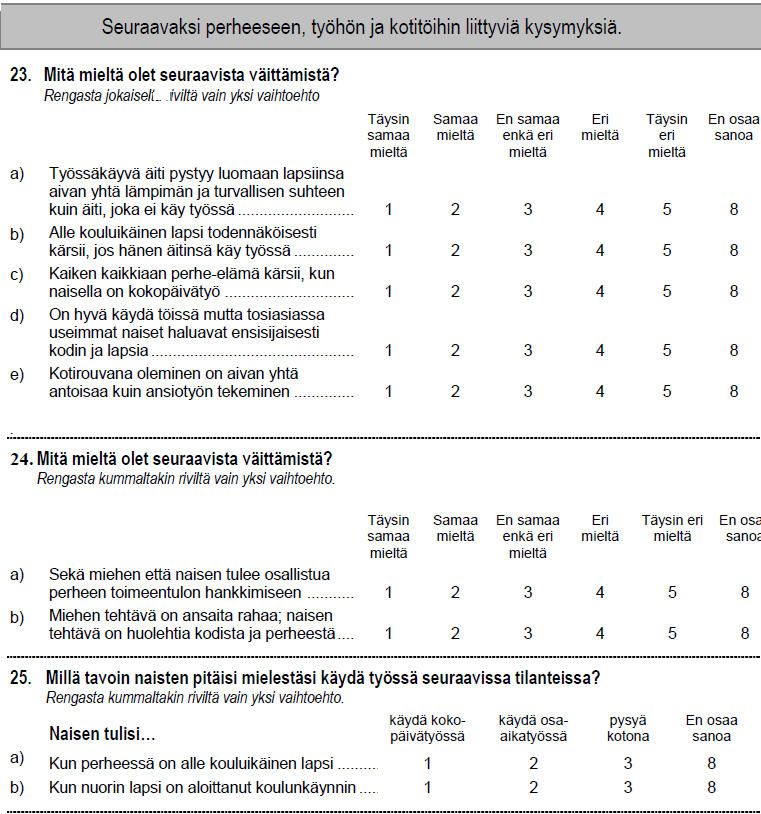
\includegraphics[width=0.6\linewidth]{img/substvarfiQ1Q2} 

}

\caption{Esimerkki suomenkielisestä lomakkeesta}\label{fig:L1suomlom1}
\end{figure}

\hypertarget{r---koodi}{%
\section{R - koodi}\label{r---koodi}}

Jotenkin tänne.

\hypertarget{tekninen-ymparisto-ja-bookdown-paketti}{%
\section{Tekninen ympäristö ja
Bookdown-paketti}\label{tekninen-ymparisto-ja-bookdown-paketti}}

Muokataan tiiviimpi pätkä esimerkkireposta bookdown-testi1. Tämä kuva
kertoo vain julkaisutekniikan ympäristön.

\begin{Shaded}
\begin{Highlighting}[]
\NormalTok{knitr}\OperatorTok{::}\KeywordTok{include_graphics}\NormalTok{(}\StringTok{'img/BookdownProc.png'}\NormalTok{)}
\end{Highlighting}
\end{Shaded}

\begin{figure}

{\centering 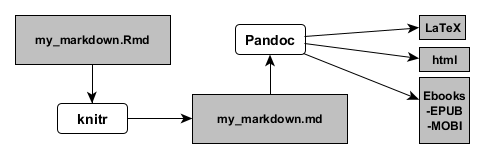
\includegraphics[width=0.6\linewidth]{img/BookdownProc} 

}

\caption{Tulostiedoston prosessointi}\label{fig:L3bdprocess1}
\end{figure}

\bibliography{jhca2018.bib,packages.bib}


\end{document}
